\section{Software Simulation}

The algorithms as described in section \ref{connectingNodes} and \ref{OptimizingNodeLocation} have been implemented and augmented with a graphical user interface (GUI). The GUI allows for the plotting of sensor (shown as white points) and relay nodes (shown as red points) and their corresponding edges in 2D-space. Figure \ref{gui} illustrates the GUI showing a graph of 11 sensor nodes and 10 relay nodes. The graph has been optimized to maximize energy consumption fairness. The GUI supports the loading and saving of nodes. Once a dataset of sensor nodes is loaded, the interface connects the nodes using the Steiner Minimum Tree approximation described in section \ref{connectingNodes}. The \textit{Action} menu item enables control over the fairness optimization algorithms described in section \ref{OptimizingNodeLocation}. The top part of the interface displays statistical information such as total power consumption and fairness in power consumption of the sensor network.

\begin{figure}[htp]
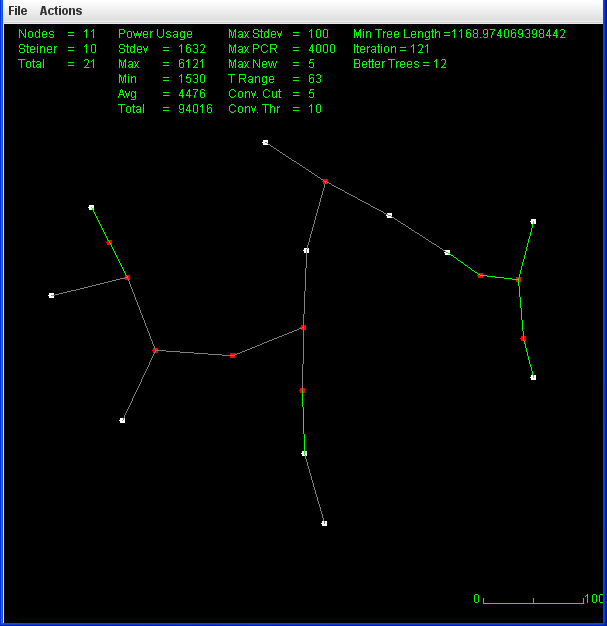
\includegraphics[scale=0.405]{images/graphical-interface.PNG}
\caption{The graphical user interface (GUI) for creating \textit{fair} sensor networks. 11 sensor (white) and 10 Relay (red) nodes are plotted in 2D-space. The image shows the resulting sensor network after optimizing energy consumption fairness.}
\label{gui}
\end{figure}